\documentclass[a4paper]{article}

\setlength{\parindent}{0pt}
\setlength{\parskip}{1em}

\pagestyle{headings}

\usepackage{amssymb}
\usepackage{amsmath}
\usepackage{amsthm}
\usepackage{mathtools}
\usepackage{graphicx}
\usepackage{hyperref}
\usepackage{color}
\usepackage{microtype}
\usepackage{tikz}
\usepackage{pgfplots}
\usepackage{pgfplotstable}

\newcommand{\N}{\mathbb{N}}
\newcommand{\Q}{\mathbb{Q}}
\newcommand{\Z}{\mathbb{Z}}
\newcommand{\R}{\mathbb{R}}
\newcommand{\C}{\mathbb{C}}
\newcommand{\D}{\mathcal{D}}
\renewcommand{\S}{\mathcal{S}}
\renewcommand{\P}{\mathbb{P}}
\newcommand{\F}{\mathbb{F}}
\newcommand{\E}{\mathbb{E}}
\newcommand{\bra}{\langle}
\newcommand{\ket}{\rangle}


\graphicspath{{Image/}}

\hypersetup{
    colorlinks=true,
    linktoc=all,
    linkcolor=blue
}

\theoremstyle{definition}
\newtheorem*{axiom}{Axiom}
\newtheorem*{claim}{Claim}
\newtheorem*{conv}{Convention}
\newtheorem*{coro}{Corollary}
\newtheorem*{defi}{Definition}
\newtheorem*{eg}{Example}
\newtheorem*{lemma}{Lemma}
\newtheorem*{notation}{Notation}
\newtheorem*{prob}{Problem}
\newtheorem*{post}{Postulate}
\newtheorem*{prop}{Proposition}
\newtheorem*{rem}{Remark}
\newtheorem*{thm}{Theorem}

\DeclareMathOperator{\vdiv}{div}
\DeclareMathOperator{\grad}{grad}
\DeclareMathOperator{\curl}{curl}
\DeclareMathOperator{\Ann}{Ann}
\DeclareMathOperator{\Fit}{Fit}
\DeclareMathOperator{\Diag}{Diag}
\DeclareMathOperator{\tr}{tr}
\DeclareMathOperator{\im}{im}
\DeclareMathOperator{\Mat}{Mat}
\DeclareMathOperator{\Log}{Log}
\DeclareMathOperator{\Isom}{Isom}
\DeclareMathOperator{\Mesh}{Mesh}
\DeclareMathOperator{\Sym}{Sym}
\DeclareMathOperator{\Aut}{Aut}
\DeclareMathOperator{\cosech}{cosech}
\DeclareMathOperator{\Card}{Card}
\DeclareMathOperator{\Gal}{Gal}


\setcounter{section}{-1}

\begin{document}

\title{Applied Probability}

\maketitle

\newpage

\tableofcontents

\newpage

\section{Miscellaneous}

Some speech

Google lecture's name to find his homepage and example sheets or probably some notice of a change of room

\newpage

\section{Poisson process}

Suppose we have a Geiger counter. We model the "click process" as a family $\{N(t) : t \geq 0\}$, where $N(t)$ denotes the total number of ticks up to time $t$. Now note that $N(t) \in \{0,1,...\}$, $N(s) \leq N(t)$ if $s \leq t$, $N$ increases by unit jumps, and $N(0) = 0$. We also assert that $N$ is right-continuous, i.e. $\lim_{x \to t^+} N(x) = N(t)$.

\begin{defi} (infinitesimal definition)\\
A \emph{Poisson process} with intensity $\lambda$ is a process $N=(N(t):t \geq 0)$ which takes values in $S = \{0,1,2,...\}$, s.t.:\\
(a) $N(0) = 0$, $N(s) \leq N(t)$ if $s \leq t$;\\
(b) 
\begin{equation*}
\begin{aligned}
\P(N(t+h)=n+m | N(t) = n) = \left\{\begin{array}{ll}
\lambda h + o(h) & m=1\\
o(h) & m>1\\
1-\lambda h & m=0
\end{array}
\right.
\end{aligned}
\end{equation*}
Recall that $g(h) = o(h)$ means that $\frac{g(h)}{h} \to 0$ as $h \to 0$;\\
(c) if $s<t$, then $N(t)-N(s)$ is independent of all arrivals prior to $s$.
\end{defi}

\begin{thm}
$N(t)$ has the Poisson distribution with parameter $\lambda t$.
\begin{proof}
Study $N(t+h)$ given $N(t)$. We have 
\begin{equation*}
\begin{aligned}
\P(N(t+h) =j) &= \sum_{i\leq j} \P(N(t+h) \\
&= j|N(t) = i) \P(N(t) = i) \\
&= (1-\lambda h) \P(N(t) = j) + \lambda h \P(N(t) = h-1) + o(h)
\end{aligned}
\end{equation*}
So
\begin{equation*}
\begin{aligned}
\frac{\P(N(t+h)=j) - \P(N(t) = j)}{h} = -\lambda \P(N(t) = j) + \lambda \P (N(t) = j-1) + \frac{o(h)}{h}
\end{aligned}
\end{equation*}
write $p_n(t) = \P(N(t) = n)$, then let $h \to 0^+$ we get
\begin{equation*}
\begin{aligned}
p'_j(t) &= -\lambda p_j(t) + \lambda p_{j-1}(t) & j \geq 1\\
p'_0(t) &= -\lambda p_0(t) &
\end{aligned}
\end{equation*}
with boundary condition $p_0(0) = 1$.\\
We solve $p_0$ to get $p_0(t) = e^{-\lambda(t)}$. Then we can use this to inductively solve $p_1,p_2,...$ to get the desired result.
\end{proof}
\end{thm}

An alternative derivation from the differential equations:\\
Let $G(s,t) = \sum_j s^j p_j(t)$. Now we take the set of differential equation, multiplying each one by $s^j$, then we get
\begin{equation*}
\begin{aligned}
\frac{\partial G}{\partial t} = \lambda (s-1) G
\end{aligned}
\end{equation*}
Then we have $$G(s,t) = A(s) e^{\lambda (s-1) t}$$ We also have $G(s,0)=1$ so we should be able to plug in a suitable value of $s$ to get the desired result (I probably missed that).

\begin{defi}(Holding/interarrival times)
In a poisson process (pp) with parameter $\lambda$, let $N(t)$ denote the total number of "clicks". Define the arrival times $T_0 = 0$, $T_n = \inf \{t \geq 0: N(t) = n\}$, i.e. the first time $t$ that $N$ reaches $n$ (note right continuity of $N$). We also define the interarrival times $X_n = T_n - T_{n-1}$.
\end{defi}

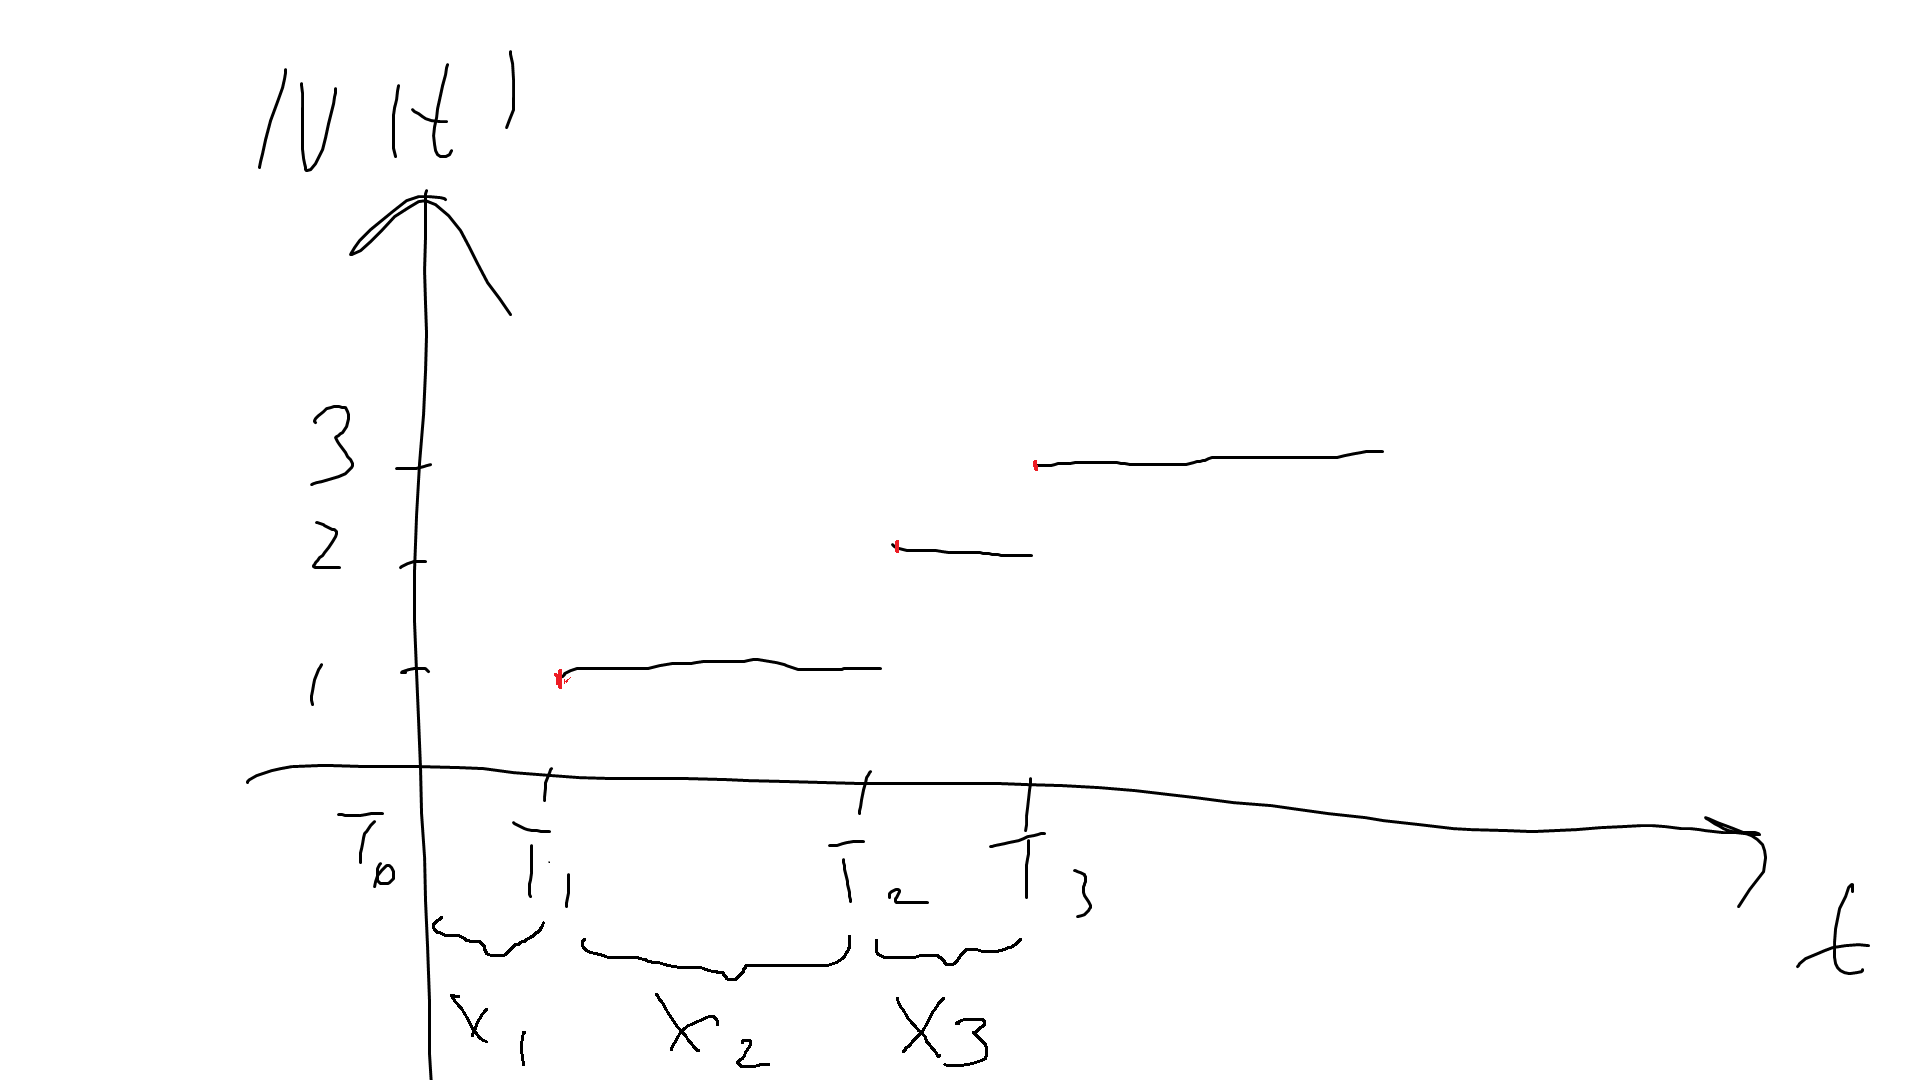
\includegraphics[scale=0.5]{image/AP_01.png}

\begin{thm}
Suppose $X_1,X_2,...$ are known. Let $T_n = \sum_1^n x_i$, note $N(t) = \max\{n:T_n \leq t\}$. Then the random variables $X_1,X_2,...$ are independent and they have the exponential distribution with parameter $\lambda$ ($Exp(\lambda)$).
\begin{proof}
\begin{equation*}
\begin{aligned}
\P(X_1 > t) = \P(N(t) = 0) = e^{-\lambda t}
\end{aligned}
\end{equation*}
So $X_1$ has $Exp(\lambda)$ distribution. Now consider $\P(X_2>t|X_1=t_1)$. This doesn't look to make much sense as $X_1$ has a continuous distribution so $\P(X_1=t_1) = 0$; however we could could consider the conditional densiy as $f_{X|Y} (x|y) =\frac{f_{X,Y}(x,y)}{f_Y(y)}$. Then $\P(X_2>t|X_1=t_1) = \P($ no arrivals in $(t_1,t_1+t)|X_1=t_1) = \P($ no arrivals in $(t_1,t_1+t)$ by independence. This is then equal to $\P($ no arrivals in $(0,t)) = \P(N(t)=0) = e^{-\lambda t}$. Then continue by induction.
\end{proof}
\end{thm}

\begin{prop} (properties of a poisson process $N$)\\
(a) $N$ has stationary independent increments, i.e.:\\
(i) If $0<t_1<...<t_n$, then $N(t_1),N(t_2)-N(t_1),...,N(t_n)-N(t_{n-1})$ are independent;\\
(ii) $N(s+t)-N(s) \xrightarrow{d} N(t)-N(0)$.\\
Amongst processes which are right continuous, non-decreasing, has only jump discontinuities of size 1, (i) and (ii) are characteristics of the Poisson process, meaning that Poisson process is the only process that has those two properties.\\
(b) Thinning:\\
Suppose insects arrive as a poisson process with parameter $\lambda$. Each insect is a mosquito with probability $\alpha$, or a skeet with probability $1-\alpha$, and the occurences of the two insects are independent. Then\\
(i) the mosquito-arrival process $F$ is a $PP(\alpha\lambda)$, 
(ii) the skeet-arrival process is $S$ a $PP((1-\alpha)\lambda)$, and 
(iii) these processes are independent.
\begin{proof}
(i) and (ii) are immediate by infinitestimal definition of a poisson process. For (iii), by independence we mean that $\P(F(t_1)=f_1,S(t_1)=s_1,...,F(t_n)=f_n,S(t_n)=s_n) = \P(F(t_1)=f_1,...,F(t_n)=f_n) \P(S(t_1)=s_1,...,S(t_n)=s_n)$ $\forall t_1,...,t_n,f_1,...,f_n,s_1,...,s_n)$.

The simple case is 
\begin{equation*}
\begin{aligned}
\P(F(t) = f, S(t) = s) &= \frac{(\lambda t)^{f+s} e^{-\lambda t}}{(f+s)!}{{f+s} \choose f} \alpha^f (1-\alpha)^s\\
&= \frac{(\alpha\lambda t)^f}{f!} e^{-\alpha\lambda t} \frac{((1-\alpha) \lambda t)^s}{s!} e^{-(1-\alpha)\lambda t}\\
&= \P(F(t) = f) \P(S(t) = s)
\end{aligned}
\end{equation*}
\end{proof}
(c) Superposition:\\
$F$: Flies arrive as $PP(\lambda_1)$;\\
$S$: Skeets arrive as $PP(\lambda_2)$, and these processes are independent. Then $N=F+S$ is a $PP(\lambda_1+\lambda_2)$. This follows by infinitesimal construction of $PP$.\\
(d) Given $N(t) = n$, write $\mathbf{T} = (T_1,...,T_n)$, $\mathbf{t} = (t_1,...,t_n)$, we have $f_{\mathbf{T}}(\mathbf{t} | N(t) = n) =\left(\frac{1}{t}\right)^n n! L(\mathbf{t})$, where $L(\mathbf{t})=1$ iff $t_1<t_2<...<t_n$.
\begin{proof}
Next time.
\end{proof}
\end{prop}

Let's complete the proof left last lecture.

\begin{thm}
Conditional on $\{N(t) = n\}$, the times $T_1,...,T_n$ have joint pdf
\begin{equation*}
\begin{aligned}
f_{ \mathbf{T} |N(t) = n} (\mathbf{t}) = \frac{n!}{t^n} L(\mathbf{t}) 1_{\{t_n \leq t\}}
\end{aligned}
\end{equation*}
where $L(\mathbf{t}) = 1_{\{t_1 \leq t_2 \leq ... \leq t_n\}}$.
\begin{proof}
The interarrival times $X_1,X_2,...,X_n$ have joint pdf
\begin{equation*}
\begin{aligned}
f_\mathbf{X}(\mathbf{x}) = \lambda^n \exp(-\lambda \sum_i^n x_i)
\end{aligned}
\end{equation*}
by change of variables, we now have (noting $T_i = X_1+...+X_i$)
\begin{equation*}
\begin{aligned}
f_\mathbf{T} (\mathbf{t}) = \lambda^n e^{-\lambda t_n} L(\mathbf{t})
\end{aligned}
\end{equation*}
Now for $C \subseteq \R^n$, we have
\begin{equation*}
\begin{aligned}
\P(T \in C | N(t) = n) &= \frac{\P(T \subseteq C, N(t) = n)}{\P(N(t) = n)}\\
&= \frac{1}{\P(N(t)=n)} \int_C \P(N(t)\\
&= n | \mathbf{T} = \mathbf{t} ) f_\mathbf{T} (\mathbf{t}) d \mathbf{t}\\
&= \frac{1}{\P(N(t) = n)} \int_{t_n \leq t} e^{-\lambda (t-t_n)}\lambda^n e^{-\lambda t_n} L(\mathbf{t}) d\mathbf{t}
\end{aligned}
\end{equation*}
the last equation is because we need ther to be no arrival between $t$ and $t_n$. Now the conditional pdf of $\mathbf{T}$ given $N(t) = n$ is
\begin{equation*}
\begin{aligned}
\frac{1}{(\lambda t)^n e^{-\lambda t} / n!} e^{-\lambda (t-t_n)} \lambda^n e^{-\lambda t_n} L(\mathbf{t}) = \frac{n! L(\mathbf{t})}{t^n} 1_{\{t_n \leq t\}}
\end{aligned}
\end{equation*}
I think somewhere in this proof we used $\P(X \in C) = \int_C g(u) du \iff f_X(u) = g(u)$, otherwise the lecture wouldn't have written this down on a separate board.
\end{proof}
\end{thm}

\newpage

\section{Continuous-time Markov chains}

This is actually quite a complicated topic, so we are going to make a lot of assumptions to simplify it.

Assume state space $S$ is countable, and we often take $S \subseteq \Z = \{ ...,-1,0,1,...\}$ (sometimes useful to assume $|S|<\infty$).

\begin{defi}
A process $X = \{X(t) : t \geq 0\}$ taking values in $S$ satisfies the \emph{Markov property} if:\\
\begin{equation*}
\begin{aligned}
\P(X(t_n) = j| X(t_1) &= i_1,...,X(t_{n-1}) = i_{n-1}) \\
&= \P(X(t_n) = j| X(t_{n-1}) = i_{n-1})
\end{aligned}
\end{equation*}
for all $i_1,i_2,...,i_{n-1}, j \in S, t_1< t_2 < ... < t_n$.

We have the transition probabilities $p_{i,j}(s,t) = \P(X(t) = j| X(s) = i)$. We, however, assume the process is homogeneous, i.e. $$p_{i,j}(s,t) = p_{i,j} (0,t-s) := p_{i,j}(t-s) \forall s,t,i,j$$so the transition probabilities only depend on the duration of time passed instead of the absolute time. We can then write this as a transition matrix $(p_{i,j}(t))_{i,j \in S}=P_t$.
\end{defi}

\begin{prop}
The family $\{P_t: t \geq 0\}$ satisfies\\
(a) $P_0 = I$;\\
(b) $P_t$ is a \emph{stochastic} matrix, i.e. a non-negative matrix with row sum 1;\\
(c) $P_{s+t} = P_s P_t$ for $s,t \geq 0$.
\begin{proof} (of (c))\\
$p_{i,j}(s+t) = \sum_{k \in S} p_{i,k}(s)p_{j,k}(t)$ by Markov Property which is just the component form of $P_{s+t} = P_s P_t$.\\
$P_{s+t} = P_s P_t$ is sometimes called the \emph{semigroup property} ($s,t \geq 0$).\\
$(P_t:t \geq 0)$ is called a \emph{stochastic semigroup}.
\end{proof}
\end{prop}

General theory involves conditions of regularity.

We assume $X$ is a right-continuous jump process.

Holding times for general chains:

Assume $X(t_0) = i$.\\
Let $H=\inf\{t>t_0:X(t) \neq i\}$. We have $$\P(H>u+v|H>u) = \P(H>v) \ (*)$$ by Markov Property ($u,v \geq 0$).\\
Let $G(u) = \P(H>u)$. By (*), we get $\frac{G(u+v)}{G(u)} = G(v)$, so $G(u+v) = G(u)G(v)$.\\
We know $G(0) = 1$, and $G$ is non-increasing.\\
Solution: $G(n) = G(1)G(n-1) = G(1)^n$ $\forall n \in \N$. Also $G(p/q)... G(p/q) =G(p) = G(1)^p$ so $G(p/q) = G(1)^{p/q}$, hence $G(u) = G(1)^u$ for $u \geq 0$. We deduce that $G(u) = e^{-\alpha u}$ for some $\alpha>0$.

\begin{lemma}
A random variable $X>0$ has an exponential distribution iff it has the \emph{lack of memory property}: $\P(X>u+v|X>u) = \P(X>v)$ $\forall u,v > 0$.
\end{lemma}

A MC s a combination of exponential-distribution holding times, and a transition matrix for the \emph{jump chain} $Y=(Y_n)$ given by $Y_0 =X(0)$, $Y_1 = X(T_1)$, where $T_1 = \inf\{t:X(t) \neq X(0)\}$, and $Y_n = X(T_n)$ where $T_{n+1} = \inf \{t > T_n: X(t) \neq X(T_n)\}$. $Y$ is a \emph{discrete-time Markov chain.}

If in staet $i$, want $H$, we jump to state $j\neq i$ with probability $\frac{g_{ij}}{\alpha_i}$. Intensity of a jump is $\alpha_i$, and intensity of a jump to state $j$ is $g_{ij}$.\\
Note a transition from $i$ to itself is not deemed to be a transition.

We have $p_{ij} (h) = g_{ij} h + o(j)$ ($j \neq i$), $p_{ij}(h) = 1- \sum_{j \neq i} p_{ij}(h) = 1-h\sum_{j \neq i} g_{ij} + o(h) = 1-\alpha_i h + o(h) = 1+g_{ii} h + o(h)$, where we let $g_{ii} = -\alpha_i$. Now we let $G$ be the matrix $(g_{ij})$, with the off-diagonal terms the previous $g_{ij}$'s, but the diagonal terms $g_{ii}$ as defined just now (so as to make row sums 0). Now the off-diagonal terms are non-negative, and diagonal terms are non-positive. We call $G$ the \emph{generator} of the chain (otherwise known as the $Q$-matrix).

Conclusion: $\frac{P_t - I}{t} \xrightarrow{t \to 0^+} G$.\\
Questions of regularity: OK if $|S| < \infty$.

(?)
\begin{equation*}
\begin{aligned}
p_{ij}(t+h) &= \sum_k p_{ik}(t) p_{kj}(h)\\
&= \sum_{k \neq j} p_{ik}(t) [g_{kj} h + o(h) + p_{ij}(t) (1+g_{jj} h + o(h))\\
&= \sum_k p_{ik} (t) g_{kj}\\
&= pP_t \cdot G
\end{aligned}
\end{equation*}
this is the (Kolmogov) Forward Equation.

$p_{ij}(t+h) = \sum_k p_{ik}(h) p_{kj}(t)$, so $P't = GP_t$, called the K-Backward equation.

Interchange of limits requires justification -- it's OK if $|S| < \infty$.

Now $P'_t = P_t G$, we can rewrite this as $f'=fg$, which gives $f(t) = A e^{gt}$. So the solution should be $P_t = P_0(=I)e^{tG}$ (i.e. $=\sum_{k=0}^\infty \frac{t^k}{k!} G^k$).

In many cases, the solutoin to the forward and/or backward equation is the function $P=e^{tG}$.

A mistake has been made! The definition for holding time is wrong. It should be $H=\inf\{ t-t_0: X(t) \neq X(t_0), t > t_0\}$.

\iffalse
\begin{equation*}
\begin{aligned}

\end{aligned}
\end{equation*}
\fi
\end{document}
